\chapter{Least Squares Theory}

Bolstered from producing concrete results, attention now turns to an examination of solution methods through the lens of the \ft.

\section{Fundamental Theorem of Linear Algebra}  %    S    S    S    S    S    S    S    S    S    S    S    S  
\index{Fundamental Theorem of Linear Algebra!orthogonal decomposition}
The Fundamental Theorem is a beautiful and powerful statement which helps to organize techniques and results in linear algebra. It is the stage upon which the stories of existence and uniqueness play out.

An exemplar matrix,
  \begin{equation*}   %  =   =   =   =   =
   %\begin{split}
      \A{} = \mat{cccc}{1 & 0 & 0 & 0 \\ 0 & 1 & 0 & 0 \\ 0 & 0 & 0 & 0} \in \cmplx{3\times 4},
   %\end{split}
   %\label{eq:}
  \end{equation*}
demonstrates salient points with an immediate subspace decomposition. The matrix $\A{}$ maps 4--vectors from the domain $\cmplx{4}$ to 3--vectors in the codomain $\cmplx{3}$. One way to express the Fundamental Theorem is to say that the matrix $\A{}$ induces a 4 dimensional column space and a 3 dimensional row space. 

For this case, the domain can be described as
  \begin{equation*}   %  =   =   =   =   =
   %\begin{split}
      \cmplx{4} = \spn{ \bl{\mat{c}{1\\0\\0\\0}}, \bl{\mat{c}{0\\1\\0\\0}} } \oplus \spn{ \rd{\mat{c}{0\\0\\1\\0}}, \rd{\mat{c}{0\\0\\0\\1}} },
   %\end{split}
   %\label{eq:}
  \end{equation*}
and the codomain as
  \begin{equation*}   %  =   =   =   =   =
   %\begin{split}
      \cmplx{3} = \spn{ \bl{\mat{c}{1\\0\\0}}, \bl{\mat{c}{0\\1\\0}} } \oplus \spn{ \rd{\mat{c}{0\\0\\1}} }
   %\end{split}
   %\label{eq:}
  \end{equation*}
The symbol $\oplus$ specifies that the vectors spaces for the range and null space are orthogonal.

There are many statements of the Fundamental Theorem. One way describes the decomposition of the domain and codomain into the four fundamental subspaces:
\begin{table}[htbp]  %  T A B L E
    \caption[The Fundamental Theorem of Linear Algebra]{The Fundamental Theorem of Linear Algebra for $\aicmn$ }
    \begin{center}
    		\begin{tabular}{rlcccccccc}
    		  %
    		  domain:   & $\cmplx{n}$ & = & $\brnga{*}$ & $\oplus$ & $\rnlla{}$ \\
    		  %
    		  codomain: & $\cmplx{m}$ & = & $\brnga{}$  & $\oplus$ & $\rnlla{*}$
    		  %
      \end{tabular}
    \end{center}
  \label{tab:ftola}
  \end{table}%
Each domain space, domain and codomain, are expressed as an orthogonal decomposition of a range space and a null space.

\begin{landscape}
  \begin{table}[ht]
    \caption[The Fundamental Theorem of Linear Algebra in pictures]{The Fundamental Theorem of Linear Algebra and Least Squares for $\aicmn$}
    \begin{center}
      \begin{tabular}{crclc}
          %
          Domain &&&& Codomain \\\hline
          %
          \ \\
          %
          && Mapping &&  \\[0pt]
          %
          \multirow{3}{*}{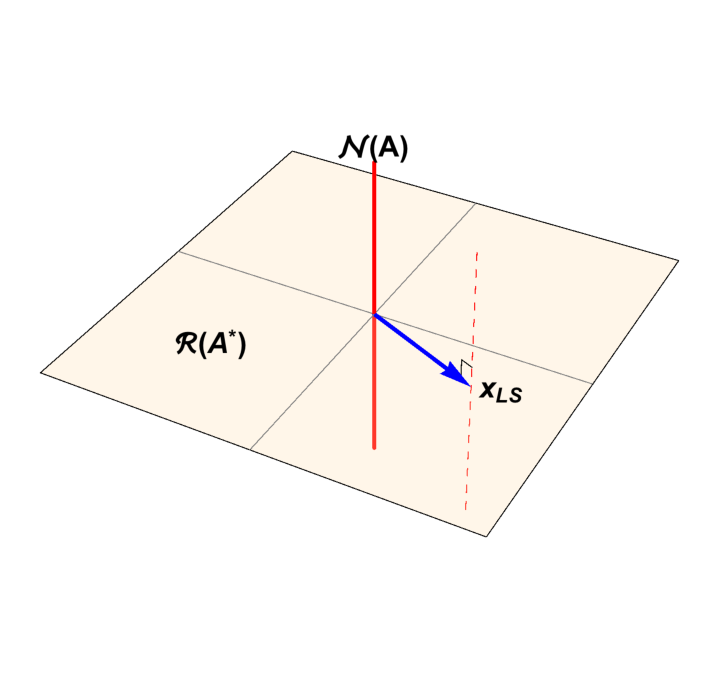
\includegraphics[ width = 2.75in ]{../pdf/theory/ftola/domain}} &&&&
          \multirow{3}{*}{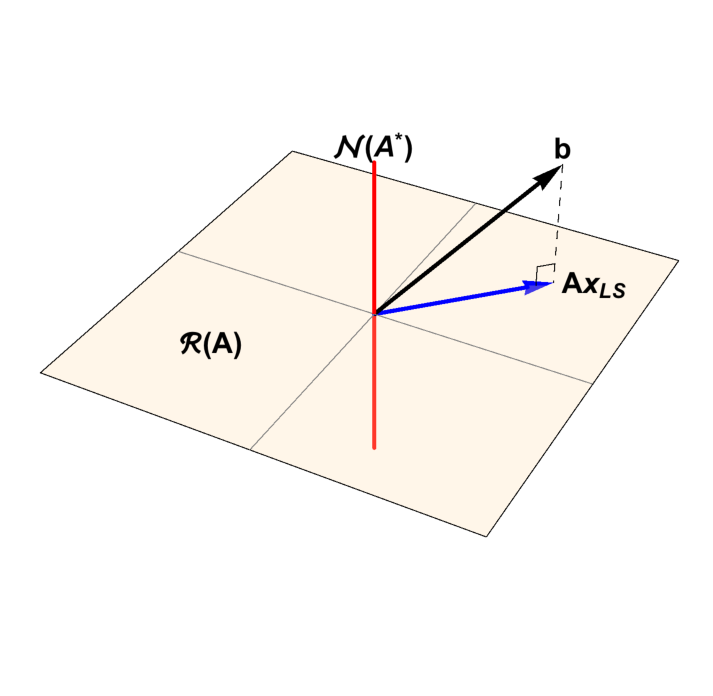
\includegraphics[ width = 2.75in ]{../pdf/theory/ftola/codomain}} \\[55pt]
            & $\A{} \colon \cmplx{n}$ & $\mapsto$ & $\cmplx{m} $ \\[15pt] 
            & $\cmplx{n}$ & $\mapsfrom$ & $\cmplx{m} \colon \A{*}$ \\[80pt]
          %
            $\cmplxn = \brnga{*} \oplus \rnlla{}$ &&  && $\cmplxm = \brnga{} \oplus \rnlla{*}$
          %
      \end{tabular}
    \end{center}
  \end{table}
\end{landscape}

  \begin{table}[htbp]  %  T A B L E
    \caption{Dimensions of the fundamental subspaces for $\aicmnr$.}
    \begin{center}
      \begin{tabular}{rclcrcl}
        %
        $\dim \paren{\brnga{}}$ & = & $\rho$ && $\dim \paren{\rnlla{*}}$ & = & $m - \rho$ \\
        %
        $\dim \paren{\brnga{*}}$ & = & $\rho$ && $\dim \paren{\rnlla{}}$ & = & $n - \rho$ 
        %
      \end{tabular}
    \end{center}
  %\label{tab:?}
  \end{table}%

Example from \eqref{eq:zonalls}

  \begin{equation*}   %  =   =   =   =   =
    \mat{rrr}{ 
      -1 & 1 & 0 \\
       0 & -1 & 1 }
  \end{equation*}
Begin with the column space, also known as the solution space because the solution parameters will inhabit this space:
  \begin{equation*}   %  =   =   =   =   =
      \text{Column vectors = } \bl{\mat{r}{ -1 \\ 0 }}, \bl{\mat{r}{ 1 \\ -1 }}, \bl{\mat{r}{ 0 \\ 1 }} .
  \end{equation*}
The column vectors are a complete span of $\cmplx{2}$, and the null space is trivial:
  \begin{equation*}   %  =   =   =   =   =
      \cmplx{2} = \spn { \bl{\mat{r}{ -1 \\ 0 }}, \bl{\mat{r}{ 1 \\ -1 }}, \bl{\mat{r}{ 0 \\ 1 }} } \mg{\oplus \mat{c}{0 \\ 0 } }
  \end{equation*}
A minimal span for $\cmplx{2}$ is
  \begin{equation*}   %  =   =   =   =   =
      \cmplx{2} = \spn { \bl{\mat{r}{ 1 \\ 0 }}, \bl{\mat{r}{ 0 \\ 1 }} }.
  \end{equation*}

Next up is the row space, or the measurement space
  \begin{equation*}   %  =   =   =   =   =
      \text{Row vectors = } \bl{\mat{r}{ -1 \\ 1 \\ 0 }}, \bl{\mat{r}{ 0  \\ -1 \\ 1 }}
   %\label{eq:}
  \end{equation*}

  \begin{equation*}   %  =   =   =   =   =
      \cmplx{3} = \spn { \bl{\mat{r}{ -1 \\ 1 \\ 0 }}, \bl{\mat{r}{ 0 \\ -1 \\ 1 }} } \oplus \spn { \rd{\mat{c}{1 \\ 1 \\1}}}
  \end{equation*}

\section{\bsvd\ - I}  %    S    S    S    S    S    S    S    S    S    S    S    S
The Fundamental Theorem describes the world as a orthogonal decomposition of the domain and codomain. Why not ask for an orthonormal decomposition? This is precisely what we get from the \asvd.
As noted by Gene Golub, the \asvd \ is a singularly valuable decomposition. It not only finds an orthonormal basis for the fundamental subspaces, it also aligns the domain and codomain, and furthermore, resolves the scale factors needed to move between spaces. This first presentation offers a statement of the SVD theorem.

\subsection{\label{ssec:SVD Theorem}SVD Theorem}  %   SS   SS   SS   SS   SS   SS   SS   SS   SS   SS   SS   SS
Given a matrix $\aicmnr$, a matrix with complex entries with $m$ rows, $n$ columns, and matrix rank $0<\rho\le\min\paren{m,n}$, then there exists a decomposition of the form
  \begin{equation}   %  =   =   =   =   =
  %\begin{split}
    \svdk{*}
    \label{eq:svdk}
  %\end{split}
  \end{equation}
where
\begin{enumerate}
  \item column vectors of unitary matrix $\V{}\icnn$ represent an orthonormal span of the domain,
  \item column vectors of unitary matrix $\U{}\icmm$ represent an orthonormal span of the codomain,
  \item Diagonal entries of $\sig{}\irmn$ contain the singular values; the ordered, nonzero eigenvalues of the product matrix $\wx{*}$.
\end{enumerate}

In block form
  \begin{equation*}   %  =   =   =   =   =
  %\begin{split}
    \A{} = \svd{*} = \csvdblockb{*}
    \label{eq:svd block}
  %\end{split}
  \end{equation*}
Column vectors span the subspaces:
  \begin{equation*}   %  =   =   =   =   =
  \begin{split}
    \V{} &= \vcols,	\\
    \U{} &= \ucols.
    %\label{eq:}
  \end{split}
  \end{equation*}
  \begin{equation*}   %  =   =   =   =   =
  \begin{split}
    \U{} & \icmm , \\
    \V{} & \icnn , \\
    \sig{} & \irmn.
    %\label{eq:}
  \end{split}
  \end{equation*}
  \begin{table}[htbp]  %  T A B L E
    \caption{Orthonormal spans for the invariant subspaces.}
    \begin{center}
      \begin{tabular}{cclcccl}
        %
        && domain &&&& codomain \\\hline
        %
        $\brnga{*}$ &=& span$\lst{\bvo, \dots, \bvrho}$ & \qquad &
        $\brnga{}$  &=& span$\lst{\buo, \dots, \burho}$ \\
        %
        $\rnlla{}$  &=& span$\lst{\rvrpo, \dots, \rvnn}$ &&
        $\rnlla{*}$ &=& span$\lst{\rurpo, \dots, \rum}$ \\
        %
      \end{tabular}
    \end{center}
  %\label{tab:?}
  \end{table}%
  
  \begin{equation*}   %  =   =   =   =   =
  \begin{split}
    u_{j} \cdot u_{k} &= \delta_{jk}, \\
    v_{j} \cdot v_{k} &= \delta_{jk}.
    %\label{eq:}
  \end{split}
  \end{equation*}

Decomposition for \eqref{eq:zonalls}:
  \begin{equation*}   %  =   =   =   =   =
  \begin{split}
    \A{} \phantom{mmmn} &=  \phantom{mmmmn} \U{}  \phantom{mmmnmm} \sig{} \phantom{mmmmmmmmm} \V{*} \\
    \mat{rrc}{-1 & 1 & 0 \\ 0 & -1 & 1} &= 
    \frac{1}{\sqrt{2}} \mat{rc}{\bmo & \bone \\ \bone & \bone }
    \mat{cc|c}{\sqrt{3} & 0 & 0 \\ 0 & 1 & 0}
    \mat{rrc}{
    \bl{\frac{1}{\sqrt{6}}}  & \bl{-\frac{2}{\sqrt{6}}} & \bl{\frac{1}{\sqrt{6}}} \\
    \bl{-\frac{1}{\sqrt{2}}} & \bl{0 \phantom{.}}       & \bl{\frac{1}{\sqrt{2}}} \\
    \rd{\frac{1}{\sqrt{3}}}  & \rd{\frac{1}{\sqrt{3}}}  & \rd{\frac{1}{\sqrt{3}}}
    }
    %\label{eq:}
  \end{split}
  \end{equation*}

  \begin{equation*}   %  =   =   =   =   =
  %\begin{split}
    \ess{} = \mat{cc}{\sqrt{3} & 0 \\ 0 & 1}
    %\label{eq:}
  %\end{split}
  \end{equation*}

\subsection{\label{SVD and Least Squares}SVD and Least Squares}  %   SS   SS   SS   SS   SS   SS   SS   SS   SS   SS   SS   SS
A direct implication of the \asvd \ is the homogeneous solution.

\subsubsection{Unitary transformation}  %  SSS  SSS  SSS  SSS  SSS  SSS  SSS  SSS  SSS  SSS  SSS  SSS
The definition of the least squares problem in \eqref{eq:xlsdef} shows that the target of minimization is the quantity
\begin{equation*}
  \rtr{*} = r^{2} = \bminimum .
\end{equation*}
One minimization strategy invokes a unitary transformation to create a simpler problem:
\begin{equation}
  \begin{split} 
    \bminimum 
      &= \normts{ \U{*} \paren{ \bl{\Ax} - b }  }.
  \end{split} 
\end{equation}
This remarkable insight opens a door to solution. Rearranging the \asvd 
\begin{equation*}
  \U{*} \A{} = \sig{} \, \V{*},
\end{equation*}
and using the block form in \eqref{eq:svd block} leads to
\begin{equation*}
  \begin{split} 
    \bminimum 
        = \normts{ \sig{} \, \V{*} x - \U{*} b }
      & = \normts{ \sbb{} \, \cvblockfs{*} x - \cublockfs{*} b } \\
	  & = \normts{ \mat{c}{ \ess{} \bvr{*} x \\[3pt]\hline\zero  } - \mat{c}{ \bur{*} b \\[3pt]\hline \run{*} b } }.
  \end{split} 
\end{equation*}
The range space components are now untangled from the  \ns \ components.

\subsubsection{Pseudoinverse solution}  %  SSS  SSS  SSS  SSS  SSS  SSS  SSS  SSS  SSS  SSS  SSS  SSS
Using the Pythagorean theorem\index{Pythagorean theorem} to isolate the range and \ns \ components of the total error for the least squares problem
\begin{equation*}
  \bminimum = \underbrace{\normts{ \ess{} \bvr{*} x -\bur{*} b  }}_{\substack{x \text{ dependence}\\\text{under control}}} + \underbrace{\normts{ \run{*} b  }}_{\substack{\text{residual}\\\text{no control}}}
\end{equation*}
There are now two terms; the first depends upon the solution vector $x$, the second does not. We only have control over the first term. To minimize the total error we must drive the first term to zero. Then the total error will be given by the residual error\index{least squares!residual error!\ns\ terms} term.
The error term that is controlled by the solution vector $x$ is this
\begin{equation}
  \ess{} \bvr{*} x - \bur{*} b .
\end{equation}
Choosing the vector $x$ which forces this term to zero  leads to the SVD solution\index{least squares!solution!SVD} for the least squares problem:
\begin{equation*}
  \xmp = \bvr{} \ess{-1} \bur{*} b.
  \label{eq:svd soln}
\end{equation*}
This is also the pseudoinverse solution\index{least squares!solution!pseudoinverse}
\begin{equation*}
  \xmp = \bl{\Ap b}
\end{equation*}
where the (thin) pseudoinverse is
\begin{equation*}
  \Ap = \bvr{} \ess{-1} \bur{*}.
  \label{eq:mpptsvd}
\end{equation*}
The error that can be controlled is forced to 0; but this leaves an error which cannot be removed, a residual error defined as
  \begin{equation*}   %  =   =   =   =   =
  %\begin{split}
    r^{2} = \normts{ \run{*} b  } .
    \label{eq:r2ub}
  %\end{split}
  \end{equation*}
The usually silent \ns \ term can be heard as it pronounces the value of the total error.

To recap, the \asvd \ leads immediately to the pseudoinverse solution and residual error.

\subsubsection{In retrospect}  %  SSS  SSS  SSS  SSS  SSS  SSS  SSS  SSS  SSS  SSS  SSS  SSS
We can reimagine the least squares problem as the challenge of resolving the data vector into range and null space components:
  \begin{equation*}   %  =   =   =   =   =
  %\begin{split}
    b = \bl{b_{\atomrng}} + \rd{b_{\atomnll}}.
    %\label{eq:}
  %\end{split}
  \end{equation*}

\begin{figure}[htbp] %  figure placement: here, top, bottom, or page
   \centering
    \begin{tikzpicture}[>=latex]
      %
      \draw [very thick] [blue!50]  [->] (0,0) -- (\scale, 0);
      \draw [very thick] [red!50]   [->] (0,0) -- (0,\scale);
      \draw [very thick] [black]    [->] (0,0) -- (\xresult,\yresult);
      %
      \draw [very thick] [blue]     [->] (0,0) -- (\xresult, 0);      
      \draw [very thick] [red]      [->] (\xresult, 0) -- (\xresult,\yresult);      
      %
      \draw [black] ( 0, \bx ) -- ( \bx, \bx );
      \draw [black] ( \bx, 0 ) -- ( \bx, \bx );
      %
      \node [] at ( \xresult - 0.25, \yresult + 0.25 ) {$b$};
      \node [] at ( \xresult + 0.5, \yresult - 0.25) {$\rd{b_{\atomnll}}$};
      \node [] at ( \xresult - 0.5, 0 + 0.35 ) {$\bl{b_{\atomrng}}$};
      %
      \node [] at ( \scale / 2, \yresult + 2.75 ) {Measurement space};
      \node [] at ( \scale / 2, \yresult + 2 ) {$\cmplxm = \brnga{} \oplus \rnlla{*}$};
      %
      \node [] at ( \scale - 0.25, 0.35 ) {$\brnga{}$};
      \node [] at ( 0.75, \scale - 0.15 )    {$\rnlla{*}$};
      \node [] at ( \scale / 2 + 1, \yresult / 2 - 0.75 ) {$b = \bl{b_{\atomrng}} + \rd{b_{\atomnll}}$};
      %
    \end{tikzpicture}
   \caption{Decomposing the data vector.}
   \label{fig:decomposing data vector}
\end{figure}
Such an example is shown in \eqref{eq:archetype:data vector}.

  \begin{equation*}   %  =   =   =   =   =
  %\begin{split}
    \normts{ \bl{\Ax} - b } = \normts{ \bl{\Ax} - \bl{b_{\atomrng}} - \rd{b_{\atomnll}} } = \normts{ \rd{b_{\atomnll}} }
    %\label{eq:}
  %\end{split}
  \end{equation*}
Because the vector $\bl{b_{\atomrng}} \in \brnga{}$, there exists a vector $x$ such that $\bl{\Ax} = \bl{b_{\atomrng}}$. Again, the error that cannot be removed is the residual error
  \begin{equation*}   %  =   =   =   =   =
  %\begin{split}
    \normts{ \rd{b_{\atomnll}} }
    %\label{eq:}
  %\end{split}
  \end{equation*}
What we shown is that the vector $x$ which minimizes the least squares error in \eqref{eq:lsmin} is exactly the same vector given by the SVD solution in equation \eqref{eq:svd soln}. Using a unitary transform we were able to convert the general least squares problem into a form amenable to solution using the \asvd.

For the overdetermined case as we have here the usually silent \ns \ term can be heard as it pronounces the value of the total error
\begin{equation}
  r^{2} = \normts{ \run{*} b  } = \paren{ \run{*} b  }^{*} \paren{ \run{*} b  } = b^{*} \paren{ \run{}\run{*} } b ,
  \label{eq:r2:a}
\end{equation}
a restatement of \eqref{eq:r2ub}.

\section{\bsvd\ - II}  %    S    S    S    S    S    S    S    S    S    S    S    S
We have a statement of the \asvd \ in \S \ref{ssec:SVD Theorem}. We have an understanding that the SVD revolves the four fundamental subspaces and the scaling factors between range spaces (eq. \eqref{eq:svdk}). We saw in \S \ref{SVD and Least Squares} how the SVD naturally leads to the pseudoinverse solution for the least squares problem. Now we turn attention to manipulation of the SVD to further explore the least squares method.

\subsection{$\sig{}$ Gymnastics}  %   SS   SS   SS   SS   SS   SS   SS   SS   SS   SS   SS   SS
Success in manipulating the \asvd \ builds	upon success in manipulating the $\sig{}$ matrices. There are three flavors of interest: the raw $\sig{}$ matrix, the transpose of this matrix, $\sig{T}$, and the pseudoinverse $\sig{\sym}$.

Think of the $\sig{}$ matrix as a sabot matrix for the matrix of singular values $\ess{}$. The padding of 0's provides compatibility of shape: the domain matrix $\U{}$ in $m \times m$; the domain matrix $\V{}$ is $n \times n$. Conformability insists the $\sig{}$ matrix in the triple product $\svds{*}{}$ have dimension $m \times n$.

The breakdown of block diagrams: the matrix $\sig{}$ $\paren{m \times n}$ and the matrix $\sig{T}$ $\paren{n \times m}$ have different shapes, but equivalent block diagrams.
  \begin{equation*}   %  =   =   =   =   =
    \begin{split}
      \sig{}  &= \mat{cc}{\ess{} & \zero \\ \zero & \zero }, \\
      \sig{T} &= \mat{cc}{\ess{T} & \zero \\ \zero & \zero } = \mat{cc}{\ess{} & \zero \\ \zero & \zero }, \\
      \sig{\sym} &= \mat{cc}{\ess{-1} & \zero \\ \zero & \zero }.
    \end{split}
   %\label{eq:}
  \end{equation*}

  \begin{equation*}   %  =   =   =   =   =
    \begin{split}
       \sig{} = 
         \mat{c|c}{\ess{}_{\rho \times \rho} & \zero_{\rho \times n-\rho} \\\hline \zero_{m-\rho \times \rho} & \zero_{m-\rho \times n-\rho} } \\
    \end{split}
   %\label{eq:}
  \end{equation*}
 There are two basic forms of interest: 

Notice the interchange of the indices $m$ and $n$ in the transpose:
  \begin{equation*}   %  =   =   =   =   =
    \begin{split}
       \sig{T} = 
         \mat{c|c}{\ess{}_{\rho \times \rho} & \zero_{\rho \times m-\rho} \\\hline \zero_{n-\rho \times \rho} & \zero_{n-\rho \times m-\rho} }.
    \end{split}
   %\label{eq:}
  \end{equation*}

The pseudoinverse matrix has the same dimension as the parent matrix:
  \begin{equation*}   %  =   =   =   =   =
    \begin{split}
       \sig{} = 
         \mat{c|c}{\ess{}_{\rho \times \rho} & \zero_{\rho \times n-\rho} \\\hline \zero_{m-\rho \times \rho} & \zero_{m-\rho \times n-\rho} } \\
    \end{split}
   %\label{eq:}
  \end{equation*}

  \begin{equation*}   %  =   =   =   =   =
    \begin{split}
      \spa &= \II{m,\rho}, \\
      \spb &= \II{n,\rho}.
    \end{split}
   %\label{eq:}
  \end{equation*}

  \begin{equation*}   %  =   =   =   =   =
   \begin{split}
   		%
       \sig{} = 
        \mat{cc}{ \sigma_{1} & 0 \\ 0 & \sigma_{2} \\ 0 & 0 \\ 0 & 0 }, \quad
        %
      \sig{T} &= 
        \mat{cccc}{ \sigma_{1} & 0 & 0 & 0 \\ 0 & \sigma_{2} & 0 & 0 }, \\
        %
      \sig{\sym} &= 
        \mat{cccc}{ 1 / \sigma_{1} & 0 & 0 & 0 \\ 0 & 1 / \sigma_{2} & 0 & 0  } .
        %
   \end{split}
    %\label{eq:}
  \end{equation*}

Stencil matrices
  \begin{equation*}   %  =   =   =   =   =
    \begin{array}{lcc ccc ccc}
      \sig{} \sig{\sym} &=& \II{4,2} &=&
        \mat{cccc}{1 & 0 & 0 & 0 \\ 0 & 1 & 0 & 0 \\ 0 & 0 & 0 & 0 \\ 0 & 0 & 0 & 0 } &=& 
        \mat{cc}{\I{2} & \zero \\ \zero & \zero }, \\ 
      \sig{\sym} \sig{} &=& \II{2,2} &=& \idtwo &=& \I{2}.
    \end{array}
   %\label{eq:}
  \end{equation*}

Product matrices with the transpose
  \begin{equation*}   %  =   =   =   =   =
    \begin{array}{lcc ccc}
      \sig{} \sig{T} &=& 
        \mat{cccc}{\sigma_{1}^{2} & 0 & 0 & 0 \\ 0 & \sigma_{2}^{2} & 0 & 0 \\ 0 & 0 & 0 & 0 \\ 0 & 0 & 0 & 0} &=& 
        \mat{cc}{\ess{2} & \zero \\ \zero & \zero }, \\
      \sig{T} \sig{} &=& 
        \mat{cc}{\sigma_{1}^{2} & 0 \\ 0 & \sigma_{2}^{2}} &=& \ess{2}.
    \end{array}
   %\label{eq:}
  \end{equation*}

Product matrices with the pseudoinverse
  \begin{equation*}   %  =   =   =   =   =
    \begin{array}{lcccccc}
      %
      \sig{} \sig{\sym} &=& \II{2,2} &=&
        \idtwo &=&
        \I{2}, \\ 
      %
      \sig{} \sig{T} &=&&& 
        \mat{cc}{\sigma_{1}^{2} & 0 \\ 0 & \sigma_{2}^{2}} &=& 
        \ess{2}, \\
      %
    \end{array}
   %\label{eq:}
  \end{equation*}

  \begin{equation*}   %  =   =   =   =   =
    \begin{array}{lcccccc}
      %
      \sig{\sym} \sig{} &=& \II{4,2} &=&
        \mat{cccc}{1 & 0 & 0 & 0 \\ 0 & 1 & 0 & 0 \\ 0 & 0 & 0 & 0 \\ 0 & 0 & 0 & 0 } &=&
        \mat{cc}{\I{2} & \zero \\ \zero & \zero }, \\ 
      %
      \sig{T} \sig{} &=&&& 
        \mat{cccc}{\sigma_{1}^{2} & 0 & 0 & 0 \\ 0 & \sigma_{2}^{2} & 0 & 0 \\ 0 & 0 & 0 & 0 \\ 0 & 0 & 0 & 0} &=& 
        \mat{cc}{\ess{2} & \zero \\ \zero & \zero }, \\
      %
    \end{array}
   %\label{eq:}
  \end{equation*}



\subsection{Fundamental Projectors}  %   SS   SS   SS   SS   SS   SS   SS   SS   SS   SS   SS   SS
Given a matrix $\aicmnr$, a matrix with complex entries with $m$ rows, $n$ columns, and matrix rank $0<\rho\le\min\paren{m,n}$, then there exists a 

\begin{table}[htbp]  % + + + + T A B L E
    \caption{Fundamental Projectors using the pseudoinverse.}
    \begin{center}
        \begin{tabular}{llclcccl}
            %
            &\multicolumn{4}{l}{Range space} & \multicolumn{3}{l}{Null space} \\\hline
            %
            domain & $\pras$ & = & $\ApA$ && $\pna$  & = & $\I{n} - \ApA$\\
            %
            codomain & $\pra$  & = & $\AAp$ && $\pnas$  & = & $\I{m} - \AAp$\\
            %
        \end{tabular}
    \end{center}
    %\label{default}
\end{table}%

\begin{table}[htbp]  % + + + + T A B L E
    \caption{Fundamental Projectors using domain matrices.}
    \begin{center}
        \begin{tabular}{llclclcl}
            %
            &\multicolumn{4}{l}{Range space} & \multicolumn{3}{l}{Null space} \\\hline
            %
            domain & $\pras$   & = & $\bvr{} \II{n,\rho} \bvr{*}$ && $\pna$   & = & $\I{n} - \bvr{} \II{n,\rho} \bvr{*}$\\
            %
            codomain & $\pra$  & = & $\bur{} \II{m,\rho} \bur{*}$ && $\pnas$  & = & $\I{m} - \bur{} \II{m,\rho} \bur{*}$\\
            %
        \end{tabular}
    \end{center}
    %\label{default}
\end{table}%

\begin{figure}[htbp] %  figure placement: here, top, bottom, or page
   \centering
    %\begin{tikzpicture}[>=stealth]
    \begin{tikzpicture}[>=latex]
      \draw [very thick] [blue!50]  [->] (0,0) -- (\scale, 0);
      \draw [very thick] [red!50]   [->] (0,0) -- (0,\scale);
      \draw [very thick] [black]    [->] (0,0) -- (\xresult,\yresult);
      %
      \draw [very thick] [blue]     [->] (0,0) -- (\xresult, 0);      
      \draw [very thick] [red]      [->] (0,0) -- (0, \yresult);      
      %
      \draw              [black] [dashed] (\xresult,0) -- (\xresult,\yresult);
      \draw              [black] [dashed] (0,\yresult) -- (\xresult,\yresult);
      %
      \draw [black] ( 0, \bx ) -- ( \bx, \bx );
      \draw [black] ( \bx, 0 ) -- ( \bx, \bx );
      %
      \node [] at ( \scale - 0.25, 0.35 ) {$\brnga{}$};
      \node [] at ( 0.75, \scale - 0.15 )    {$\rnlla{*}$};
      \node [] at ( \xresult + 0.25, \yresult ) {$b$};
      \node [] at ( \xresult - 1, 0 + 0.35 ) {$\pra{}b$};
      \node [] at ( 0.85, \yresult - 0.35 ) {$\pnas{}b$};
      \node [] at ( \scale / 2, \yresult + 2.75 ) {Measurement space};
      \node [] at ( \scale / 2, \yresult + 2 ) {$\cmplxm = \brnga{} \oplus \rnlla{*}$};
    \end{tikzpicture}
   \caption{Projections of the data vector.}
\end{figure}

\section{Least Squares Solution - Again}  %    S    S    S    S    S    S    S    S    S    S    S    S  
Let's revisit the canonical linear system in \eqref{eq:axeb} the general solution in \eqref{eq:general soln}:
  \begin{equation*}   %  =   =   =   =   =
   \begin{split}
    x_{LS} 
      &= \bsolnls{b}{y} \\
      &= \bl{\Ap b} + \pna y
   \end{split}
  \label{eq:}
  \end{equation*}
where the arbitrary vector $y\in\cmplxn$.

The projector onto the range space $\brnga{*}$
  \begin{equation*}   %  =   =   =   =   =
      \ApA = \V{}\Sigma^{\sym}\Sigma{}\V{*} = \bvr{} \II{\rho,m} \bvr{*}
 %\label{eq:}
  \end{equation*}

\section{\label{sec:reflection invariance}Reflection Invariance}  %    S    S    S    S    S    S    S    S    S
Least squares solutions have a reflection invariance based upon the arithmetic fact 
  \begin{equation*}   %  =   =   =   =   =
    \sum r_{k}^{2} = \sum \paren{-r_{k}}^{2}.
  \end{equation*}
Otherwise,
  \begin{equation*}   %  =   =   =   =   =
  %\begin{split}
    r \cdot r = \paren{-r} \cdot \paren{-r}
    %\label{eq:}
  %\end{split}
  \end{equation*}
Starting with the canonical linear system in \eqref{eq:axeb}, the least squares solution is $x_{LS}$ and the residual errors may be defined as
  \begin{equation*}   %  =   =   =   =   =
    r = \A{}x - b = r \qquad \Rightarrow \qquad r = \Ap b - b = \paren{\Ap - \I{m}}T.
  \end{equation*}
Notice that $-r = b - \Ap b$. To reflect the data points through the solution curve us
  \begin{equation*}   %  =   =   =   =   =
    \tilde{b} = b + 2r
  \end{equation*}
  \begin{equation*}   %  =   =   =   =   =
   %\begin{split}
      r = b - \A{}x 
   %\end{split}
   %\label{eq:}
  \end{equation*}

There are two equivalent ways to define the residual vector. When discussing range and null space decomposition, it is natural to write $b = \bl{b_{\atomrng}} +  \rd{b_{\atomnll}}$ as in figure \ref{fig:null up}. However, when discussing the projection of the data vector down onto the range space as in figure \ref{fig:null down}, the choice is $b +  \rd{b_{\atomnll}} = \bl{b_{\atomrng}}$. In the first instance the red arrow points up, in the second it points down.
% http://cremeronline.com/LaTeX/minimaltikz.pdf
\begin{figure}[htbp] %  figure placement: here, top, bottom, or page
   \centering
    %\begin{tikzpicture}[>=stealth]
    \begin{tikzpicture}[>=latex]
      \draw [very thick] [black] [->] (0,0) -- (9.94678, 1.03034);
      \draw [very thick] [blue]  [->] (0,0) -- (9.94678, 0);
      \draw [very thick] [red]   [->] (9.94678,0) -- (9.94678, 1.03034);
      \node[] at (5.5,1) {$b$};
			\node[] at (5.5,-0.5) {\bl{$b_{\atomrng}$}};
			\node[] at (10.5,0.5) {\rd{$b_{\atomnll}$}};
    \end{tikzpicture}
   \caption{Data vector resolved as $b = \bl{b_{\atomrng}} +  \rd{b_{\atomnll}}$.}
   \label{fig:null up}
\end{figure}

\begin{figure}[htbp] %  figure placement: here, top, bottom, or page
   \centering
    %\begin{tikzpicture}[>=stealth]
    \begin{tikzpicture}[>=latex]
      \draw [very thick] [black] [->] (0,0) -- (9.94678, 1.03034);
      \draw [very thick] [blue]  [->] (0,0) -- (9.94678, 0);
      \draw [very thick] [red]   [->] (9.94678, 1.03034) -- (9.94678, 0);
      \node[] at (5.5,1) {$b$};
			\node[] at (5.5,-0.5) {\bl{$b_{\atomrng}$}};
			\node[] at (10.5,0.5) {\rd{$b_{\atomnll}$}};
    \end{tikzpicture}
   \caption{Data vector resolved as $b +  \rd{b_{\atomnll}} = \bl{b_{\atomrng}}$.}
    \label{fig:null down}
\end{figure}


  \begin{equation*}   %  =   =   =   =   =
    \begin{split}
      x_{LS} &= x_{R} \\
      \wxi{*} \A{*} b &= \wxi{*} \A{*} \paren{b - 2r}
    %\label{eq:}
    \end{split}
  \end{equation*}
True iff $\wxi{*} \A{*} r = 0$:
  \begin{equation*}   %  =   =   =   =   =
    \begin{split}
    \wxi{*} \A{*} r 
      & = \wxi{*} \A{*} \paren{\axmb} \\
      & = \paren{\wxi{*} \wx{*}} x - \wxi{*} \A{*} b \\
      & = x - x \\
      & = \zero.
    %\label{eq:}
    \end{split}
  \end{equation*}
  
  \begin{table}[htbp]  %  T A B L E
    \caption{Reflecting the data for $\A{}x - T = r$.}
    \begin{center}
      \begin{tabular}{ccc}
        %
        method & original data & reflected data \\\hline
        %
        I & $T$  &  $T+2r$ \\
        %
        II & $\Ap a - r$ & $\Ap a + r$
        %
      \end{tabular}
    \end{center}
  %\label{tab:?}
  \end{table}%

\begin{figure}[htbp] %  figure placement: here, top, bottom, or page
   \centering
   \begin{overpic}[ scale = \myscale ]
	   {\pathgraphics "bevington plus"/"reflect bars"}
        %
      	\put(50,-3) {$a_{0}$}
      	\put(-4,33) {$a_{1}$}
	      %
   \end{overpic}
   \caption{Reflecting the data points through the solution curve.}
   \label{fig:learn:reflect}
\end{figure}

This test can be a filter as seen in \S \ref{ssec:RTF}


\endinput